% all-in-one cheatsheet layout (Michael Franzen, 2013)
\documentclass[a4paper]{article}

% geometry settings
\usepackage[top=2cm, bottom=2.5cm, left=2cm, right=2cm]{geometry}

% font settings
%\usepackage[light,math]{kurier}
\usepackage[T1]{fontenc}
\usepackage[utf8]{inputenc}
\usepackage{marvosym}
\usepackage{amssymb}
\usepackage{amsfonts}
\usepackage{amsmath}
\usepackage{amsthm}

% colors
\usepackage{xcolor}
\definecolor{lightgray}{gray}{0.8}

% formatting
\usepackage{paralist}
\usepackage{multicol}
\usepackage{tabularx}
\usepackage{Tabbing}
\usepackage{booktabs}
\usepackage{fancyhdr}
\usepackage{url}
\usepackage[framemethod=tikz]{mdframed}
\pagestyle{fancy}

% math
\usepackage{array}
\usepackage{eqnarray}
\usepackage{mathtools}

% figures
\usepackage{wrapfig}
\usepackage{subfig}

% figure modules
\usepackage{graphicx}
\usepackage{tikz}
\usetikzlibrary{positioning,calc, shapes}
\usepackage{algorithm2e}
\usepackage{verbatim}	

% TOC & Glossary
\usepackage{sectsty}
\usepackage[nottoc,notlof,notlot]{tocbibind}
\usepackage[titles,subfigure]{tocloft}

% commands
\usepackage{xargs}
\usepackage{ifthen}

% head line
\fancyhf{}
\chead{Graph Theory - Sheet 3 - \today\\J. Batzill (1698622), M. Franzen (1696933), J. Labeit (1656460)}
\renewcommand{\headrulewidth}{0.4pt} %obere Trennlinie

\newcommand{\sheetnumber}{1}

% (problem number)
\surroundwithmdframed[
    hidealllines=true,
    backgroundcolor=gray!10,
    skipbelow=\baselineskip,
    skipabove=\baselineskip
]{mylemma}

\surroundwithmdframed[
	linecolor=white,
	skipbelow=\baselineskip,
	skipabove=\baselineskip
]{mytheorem}




\begin{document}
	
	\newtheorem{mytheorem}{Theorem}[section]
	\newtheorem{mylemma}{Lemma}[mytheorem]	

	\newenvironmentx*{solution}[1]{\section*{Problem #1}\addtocounter{section}{1}\setcounter{mylemma}{0}\setcounter{mytheorem}{0}}{}
	\newenvironmentx*{theorem}[1]{\begin{mytheorem}#1\\\begin{proof}}{\end{proof}\end{mytheorem}}
	\newenvironmentx*{lemma}[1]{\begin{mylemma}#1\\\begin{proof}}{\end{proof}\end{mylemma}}


	\begin{solution}{9}
		\begin{theorem}{A hypercube $Q_n$ is Hamiltonian. It has a girth of $4$, a diameter of $n$, an order of $2^n$ and a size of ?.}
		\end{theorem}
		\begin{theorem}{A bipartite complete graph $K_{m, n}$ is Hamiltonian iff $m = n$. It's girth is $4$ for $m, n \geq 2$ and $\infty$ otherwise. It's diameter is $2$. The graph's order is $m + n$ and it's size is $m \cdot n$.}
		\end{theorem}
		\begin{theorem}{The Petersen graph is Hamiltonian, it has a girth of $5$, a diameter of $2$, an order of $10$ and a size of $15$.}
		\end{theorem}
	\end{solution}
	\newpage
	\begin{solution}{10}
		\begin{theorem}{For a natural number $n \geq 2$ let $G = (V_G, E_G)$ be the graph of order $2n + 1$ obtained from $K_{n,n}$ by subdividing an edge by a vertex. Then, $\chi'(X) = \Delta(G) + 1 = n + 1$ but $\chi'(G - e) = \Delta(G - e)$ for any edge $e$ of $G$.}
			Let $V = \{v_1, ..., v_n\}$ and $W = \{w_1, ..., w_n\}$ denote the two partitions of $K_{n, n}$ and $\{c_k\ |\ k \in \mathbb{N}\}$ be a set of colors. Furthermore, let $u \in V_G$ be the vertex subdividing an edge between these two partitions.\\
		
			First, we will prove that $\chi'(X) = \Delta(G) + 1 = n + 1$. We will argue, that any partial coloring of $G$ will inevitably result in $n+1$ colors. 
%
% noncolored graph $G$, coloring the edges incident to a vertex $v \in V$ will inevitably result in $n + 1$ colors. Since $V$ and $W$ are entirely commutable, our proof will be sufficient after we consider the extra case in which we begin with coloring the edges of $u$.

			\begin{center}
				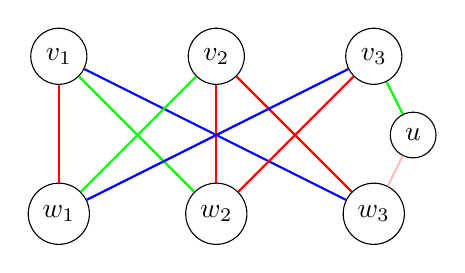
\begin{tikzpicture}
					\node[draw,circle] (v1) at (0, 0) {$v_1$};
					\node[draw,circle] (v2) at (2, 0) {$v_2$};
					\node[draw,circle] (v3) at (4, 0) {$v_3$};
					\node[draw,circle] (w1) at (0, -2) {$w_1$};
					\node[draw,circle] (w2) at (2, -2) {$w_2$};
					\node[draw,circle] (w3) at (4, -2) {$w_3$};
					\node[draw,circle] (u) at (4.5, -1) {$u$};
		
					\draw[thick, red] (v1) -- (w1);
					\draw[thick, green] (v1) -- (w2);
					\draw[thick, blue] (v1) -- (w3);
					\draw[thick, green] (v2) -- (w1);
					\draw[thick, red] (v2) -- (w2);
					\draw[thick, red] (v2) -- (w3);
					\draw[thick, blue] (v3) -- (w1);
					\draw[thick, red] (v3) -- (w2);
					\draw[thick, green] (v3) -- (u);
					\draw[thick, pink] (u) -- (w3);
				\end{tikzpicture}
			\end{center}

			For a partially colored $G$, let $v \in V_G$ be a vertex of $G$.
			\begin{itemize}
				\item \textbf{Case 1:} $v \neq u$: Since $v$ has $n$ adjacent vertices, we need $n$ colors to color the edges incident to $v$. Of course, 
			\end{itemize}
		\end{theorem}
	\end{solution} 
	\newpage
	\begin{solution}{11}
		For each even integer $k > 1$, the complete graph $K_{(n+1)}$ is a $k$-regular graph with no 1-factor. For each odd integer $k > 1$ the graph must not be bipartite (\emph{Hall's Theorem}). Furthermore, there must be a subset $U$ such that the graph without $U$ has at least $|U|$ connected components with an odd number of vertices (\emph{Tutte Theorem}).
	\end{solution} 
	\newpage
	\begin{solution}{12}
	In the following I will show that any graph $G$ with $2n$ vertices and all degrees at least $n$ has a 1-factor. 	
	I will show that if we divide such a $G$ into two parts we can remove edges until we get an bipartite 1-regular graph. 
	Then using the corollary of Hall's theorem we know we can find a perfect matching.
		\begin{theorem}{Let $G=(V,E)$ be a graph with $|V| = 2n$ vertices with all degree atleast n, then $G$ has a 1-factor.}
		Because $|V| = 2n$ we can divide the vertices $V$ into two subsets $A,B \subset V$ with $|A|=|B|=n$ and $A \cap B = \emptyset$. 
		
	
		\end{theorem}
	\end{solution}
	
\end{document}